% file thesis.tex
% Archivo thesis.tex
% Documento maestro que incluye todos los paquetes necesarios para el documento
% principal.

% Documento obtenido por un sinfin de iteraciones de administradores del LDC
% Estructura actual hecha por:
% Jairo Lopez <jairo@ldc.usb.ve>
% Actualizado ligeramente por:
% Alexander Tough 

\documentclass[oneside,12pt,letterpaper]{report}
\tolerance=1000  
\hbadness=10000  
\raggedbottom

% Para escribir algoritmos
\usepackage{listings}
\usepackage{algpseudocode}
\usepackage{algorithmicx}
\usepackage{algorithm}

\usepackage{pdflscape}

% Paquetes para manejar graficos
\usepackage{epsf}
\usepackage[pdftex]{graphicx}
\usepackage{epsfig}
% Simbolos matematicos
\usepackage{latexsym,amssymb}
% Paquetes para presentar una tesis decente.
\usepackage{setspace,cite} % Doble espacio para texto, espacio singular para
                           % los caption y pie de pagina

\usepackage[table]{xcolor}
\usepackage{tikz}
\usetikzlibrary{shapes.geometric,arrows}

\usetikzlibrary{arrows,shapes}
\usepackage{verbatim}

\usepackage{comment}

% Paquetes no utilizados para citas
%\usepackage{mcite} 
%\usepackage{draft} 

\usepackage{wrapfig}
\usepackage{alltt}

% Acentos 
\usepackage[spanish,activeacute,es-noquoting]{babel}

\usepackage[spanish]{translator}
\usepackage[utf8]{inputenc}
\usepackage{color, xcolor, colortbl}
\usepackage{multirow}
\usepackage{subfig}
\usepackage[OT1]{fontenc}
\usepackage{tocbibind}
\usepackage{anysize}
\usepackage{listings} 

% Para poder tener texto asiatico
%\usepackage{CJK}

\usepackage{pdfpages}

% Opciones para los glosarios
\usepackage[style=altlist,toc,numberline,acronym]{glossaries}
\usepackage{url}
\usepackage{amsthm}
\usepackage{amsmath}
\usepackage{fancyhdr} % Necesario para los encabezados
\usepackage{fancyvrb}
\usepackage{makeidx} % En caso de necesitar indices.
\makeindex  % Necesitado para los indices

% Definiciones para definicions, teoremas y lemas
\theoremstyle{definition} \newtheorem{definicion}{Definici\'{o}n}
\theoremstyle{plain} \newtheorem{teorema}{Teorema}
\theoremstyle{plain} \newtheorem{lema}{Lema}

% Para la creacion de los pdfs
\usepackage{hyperref}

% Para resolver el lio del Unicode para la informacion de los PDFs
% En pdftitle coloca el nombre de su proyecto de grado/pasantia.
% En pdfauthor coloca su nombre.
\hypersetup{
    pdftitle = {Desarrollo de una aplicación móvil de control y reportes de gastos},
    pdfauthor={Susana Charara Charara},
    colorlinks,
    citecolor=black,
    filecolor=black,
    linkcolor=black,
    urlcolor=black,
    backref,
    pdftex
}

\definecolor{brown}{rgb}{0.7,0.2,0}
\definecolor{darkgreen}{rgb}{0,0.6,0.1}
\definecolor{darkgrey}{rgb}{0.4,0.4,0.4}
\definecolor{lightgrey}{rgb}{0.95,0.95,0.95}

\usepackage{listings}
\lstnewenvironment{code}{\lstset{basicstyle=\small}}{}

\lstset{escapeinside=~~}
\lstset{
   frame=single,
   framerule=1pt,
   showstringspaces=false,
   basicstyle=\footnotesize\ttfamily,
   keywordstyle=\textbf,
   backgroundcolor=\color{lightgrey}
}

% Crea el glosario
%\makeglossaries

% Incluye el glosario
%\newglossaryentry{PILA}
{
  name=Pila,
  description={Es una lista en la que el modo de agregar sus elementos es de tipo 
	último en entrar, primero en salir que permite almacenar y recuperar datos.}
}

\newglossaryentry{COLA}
{
  name=Cola,
  description={Es una lista en la que el modo de agregar sus elementos es de tipo 
	primero en entrar, primero en salir que permite almacenar y recuperar datos.}
}

\newglossaryentry{ARREGLO}
{
  name=Arreglo,
  description={Es una lista ordinal en la que el modo de acceso a sus elementos 
  es indexado que permite almacenar y recuperar datos pero no modificar su
  tamaño inicial.}
}

\newglossaryentry{GRAFO}
{
  name=Grafo,
  description={Es una red que une nodos que permiten almacenar y recuperar datos.}
}


% Para crear la hoja escaneada de las firmas
\usepackage[absolute]{textpos}

% Pone los nombres y las opciones para mostrar los codigos fuentes
\lstset{language=C, breaklines=true, frame=single, showstringspaces=false,
        showtabs=false, numbers=left, keywordstyle=\color{black},
        basicstyle=\footnotesize, captionpos=b }
\renewcommand{\lstlistingname}{C\'{o}digo fuente}
\renewcommand{\lstlistlistingname}{\'{I}ndice de c\'{o}digos fuentes}

\newcommand{\todo}{ TODO: }

% Dimensiones de la pagina
\setlength{\headheight}{15pt}
\marginsize{3cm}{2cm}{2cm}{2cm}

%%%%%%%%%%%%%%%%%%%%%%%%%%%%%%%%%%%%%%%%%%%%%%%%%%%%%%%%%%%%%%%%%%%%%%%%%%%
%%%%%%%%%%%%%%%%      end of preamble and start of document     %%%%%%%%%%%
%%%%%%%%%%%%%%%%%%%%%%%%%%%%%%%%%%%%%%%%%%%%%%%%%%%%%%%%%%%%%%%%%%%%%%%%%%%
\begin{document}

% Pagina de titulo
% Pagina de titulo
\begin{titlepage}
\begin{center}

% Upper part (aqui ya esta incluido el logo de la USB).

\includegraphics[scale=0.5,type=png,ext=.png,read=.png]{imagenes/cebolla} \\

% Encabezado
\textsc {\large UNIVERSIDAD SIMÓN BOLÍVAR} \\
\textsc{\bfseries DECANATO DE ESTUDIOS PROFESIONALES\\
COORDINACI'ON DE INGENIER'IA DE LA COMPUTACI'ON}

\bigskip
\bigskip
\bigskip
\bigskip
\bigskip
\bigskip
\bigskip
\bigskip
\bigskip

% Title/Titulo
% Aqui ponga el nombre de su proyecto de grado/pasantia larga
\textsc{\bfseries DESARROLLO DE UNA APLICACIÓN MÓVIL DE CONTROL Y REPORTES DE GASTOS}

\bigskip
\bigskip
\bigskip
\bigskip
\bigskip

% Author and supervisor/Autor y tutor
\begin{minipage}{\textwidth}
\centering
Por: \\ SUSANA CHARARA CHARARA \\

\bigskip
\bigskip
\bigskip

Realizado con la asesoría de: \\
Tutor Académico: XIOMARA CONTRERAS \\
Tutor Industrial: LUIS AUGUSTO PEÑA PEREIRA
\end{minipage}

\bigskip
\bigskip
\bigskip
\bigskip
\bigskip
\bigskip
\bigskip
\bigskip
\bigskip

% Bottom half
{INFORME DE PASANTÍA LARGA \\ Presentado ante la Ilustre Universidad Simón Bolívar \\
como requisito parcial para optar al título de \\ Ingeniero en Computación} \\

\bigskip
\bigskip
\vfill

% Date/Fecha 
{\large \bfseries Sartenejas, 
%FECHA
SEPTIEMBRE de 2016}

\end{center}
\end{titlepage}

% Pagina de titulo
\begin{titlepage}
\begin{center}

% Upper part (aqui ya esta incluido el logo de la USB).

\includegraphics[scale=0.5,type=png,ext=.png,read=.png]{imagenes/cebolla} \\

% Encabezado
\textsc {\large UNIVERSIDAD SIMÓN BOLÍVAR} \\
\textsc{\bfseries DECANATO DE ESTUDIOS PROFESIONALES\\
COORDINACI'ON DE INGENIER'IA DE LA COMPUTACI'ON}

\bigskip
\bigskip
\bigskip
\bigskip
\bigskip
\bigskip
\bigskip
\bigskip
\bigskip

% Title/Titulo
% Aqui ponga el nombre de su proyecto de grado/pasantia larga
\textsc{\bfseries DESARROLLO DE UNA APLICACIÓN MÓVIL DE CONTROL Y REPORTES DE GASTOS}

\bigskip
\bigskip
\bigskip
\bigskip
\bigskip

% Author and supervisor/Autor y tutor
\begin{minipage}{\textwidth}
\centering
Por: \\ SUSANA CHARARA CHARARA \\

\bigskip
\bigskip
\bigskip

Realizado con la asesoría de: \\
Tutor Académico: XIOMARA CONTRERAS \\
Tutor Industrial: LUIS AUGUSTO PEÑA PEREIRA
\end{minipage}

\bigskip
\bigskip
\bigskip
\bigskip
\bigskip
\bigskip
\bigskip
\bigskip
\bigskip

% Bottom half
{INFORME DE PASANTÍA LARGA \\ Presentado ante la Ilustre Universidad Simón Bolívar \\
como requisito parcial para optar al título de \\ Ingeniero en Computación} \\

\bigskip
\bigskip
\vfill

% Date/Fecha 
{\large \bfseries Sartenejas, 
%FECHA
SEPTIEMBRE de 2016}

\end{center}
\end{titlepage}

% Pagina de acta final (vacio)
%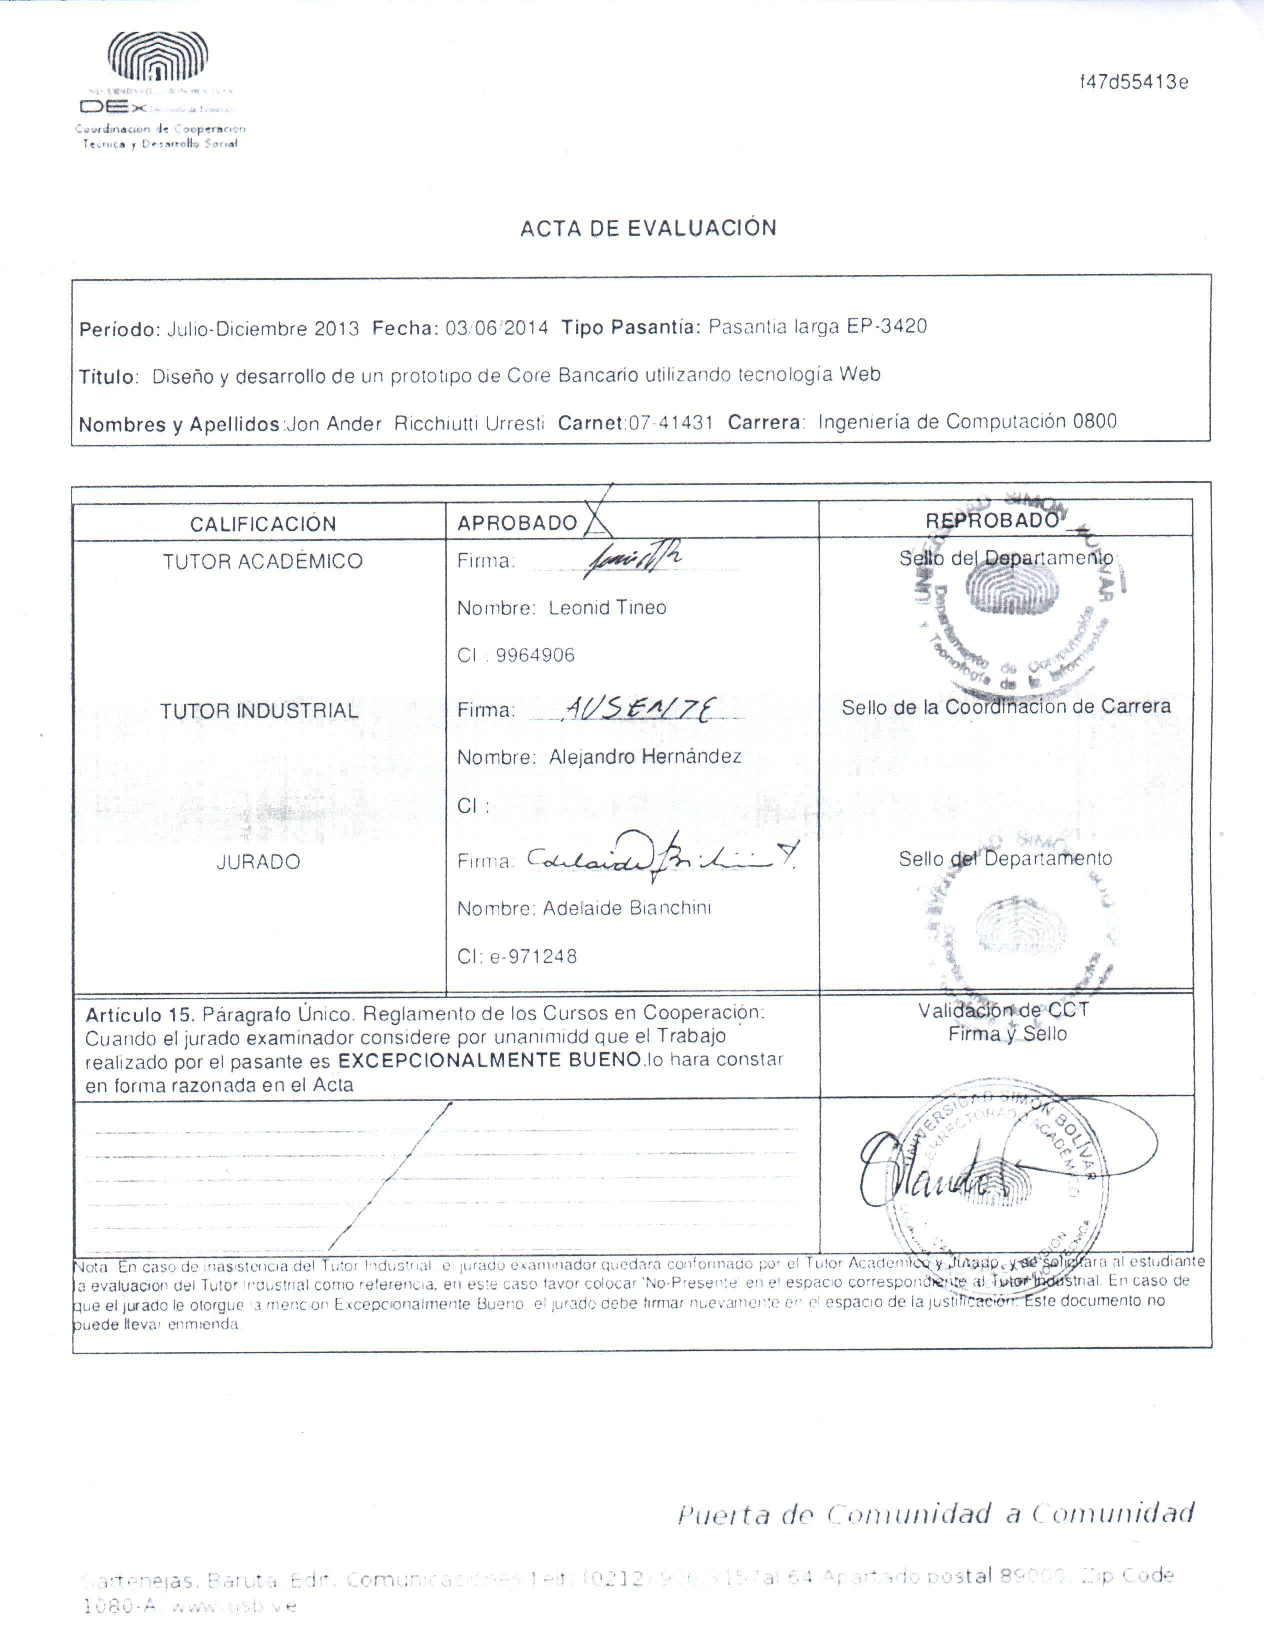
\includepdf[pages={1}]{intro/firmas.pdf}

%\setcounter{secnumdepth}{3}
%\setcounter{tocdepth}{4}

% Define encabezado numeros romanos y como se separan los captiulos y las
% secciones
\addtolength{\headheight}{3pt}
\pagenumbering{roman}
\pagestyle{fancyplain}

\renewcommand{\chaptermark}[1]{\markboth{\chaptername\ \thechapter:\,\ #1}{}}
\renewcommand{\sectionmark}[1]{\markright{\thesection\,\ #1}}

\onehalfspacing

\lhead{}
\chead{}
\rhead{}
\renewcommand{\headrulewidth}{0.0pt}
\lfoot{}
\cfoot{\fancyplain{}{\thepage}}
\rfoot{}


% Pagina de resumen
%\setcounter{page}{3}
\begin{center}
	{\bf Resumen} \pdfbookmark[0]{Resumen}{resumen} % Sets a PDF bookmark for the dedication
\end{center}	

En esta pasantía se desarrolló, para la empresa Digitalica Group, C.A., una aplicación para dispositivos móviles con la cual se pueden realizar reportes de gastos. Actualmente, la empresa Digitalica Group, C.A. ofrece a sus trabajadores el beneficio de realizar reembolsos de gastos en ciertos rubros; el proyecto nació como solución al problema de agilizar el proceso en que los trabajadores hacen llegar a los supervisores la información de estos gastos. Con la aplicación desarrollada, se pueden registrar gastos e ingresos con un monto, fecha y descripción. Se permite también capturar y guardar fotos tanto de los ingresos como de los gastos, de manera que el usuario puede tomar fotos de los recibos de sus gastos. Además, estos gastos/ingresos pueden estar asociados a categorías, que indican el rubro al que pertenecen. La aplicación permite al usuario generar archivos con formato PDF que contienen un reporte con una lista de gastos, en un rango de fecha determinado; estos reportes se pueden enviar a un servidor web. Este servidor también fue desarrollado durante la pasantía; con él, se prestan los servicios necesarios para que la aplicación pueda autenticar usuarios y enviar reportes. Igualmente, se desarrolló una aplicación web que permite a los supervisores de la empresa revisar los reportes recibidos, aprobarlos y rechazarlos.

En este informe se describen los conceptos teóricos que ayudaron al diseño y desarrollo de la solución. Igualmente, se describe el proceso de desarrollo de los tres componentes principales desarrollados durante la pasantía: aplicación nativa para Android, servidor web y aplicación web. El desarrollo de estos involucró el diseño e implementación de los modelos de datos de la aplicación y el servidor, así como múltiples interfaces de usuario que permiten la interacción con los modelos. Para cada componente, se describen el entorno de trabajo y las herramientas utilizadas. Se utilizó Java como lenguaje de programación tanto de la aplicación móvil como del servidor; entre las herramientas que se emplearon en el desarrollo del servidor se pueden mencionar AppFuse, Spring, Hibernate y Tapestry, entre otros.

Por otra parte, se utilizó Scrum como marco de trabajo, dividiendo el desarrollo del proyecto en ocho iteraciones, en las que se implementaron los componentes y funcionalidades necesarios para el cumplimiento de los objetivos de la pasantía.

El objetivo del desarrollo de la pasantía fue ofrecer una solución al problema que actualmente se presenta en la empresa de agilizar el proceso de reembolso sobre ciertos gastos.




% Pagina de dedicatoria (opcional)
%\pagebreak

%\setcounter{page}{5}

\vspace*{8cm} 
\pdfbookmark[0]{Dedicatoria}{dedicatoria} % Sets a PDF bookmark for the dedication
\begin{center} 
\large A nuestros padres.\\ Porque nos dieron la vida y nos han guiado 
a ser quienes somos hoy.
\end{center}
\newpage


% Pagina de agradecimientos (opcional)
%%\setcounter{page}{6}

\chapter*{Agradecimientos
\markboth{Agradecimientos}{Agradecimientos}}
\pdfbookmark[0]{Agradecimientos}{agradecimientos}

\bigskip



% Crea la tabla de contenidos
%\tableofcontents

% Crea la lista de cuadros
%\listoftables

% Crea la lista de figuras
%\listoffigures
%\newpage
\phantomsection
%%\setcounter{page}{4}
\chapter*{Lista de Símbolos y Abreviaturas}% Sets a PDF bookmark for the dedication

\vspace{5 mm}
\noindent
\textbf{BPM:} Business Process Management (en español Gestión de Procesos de Negocio)\\ \\

%\addcontentsline{toc}{chapter}{Lista de Símbolos y Abreviaturas}

% Crea la lista de codigos fuentes
%\lstlistoflistings

\clearpage

% Define encabezado en numeros arabicos  
\pagenumbering{arabic}

\fancyhf{} % Redefine el encabezado 
\lhead{}
\chead{}
\rhead{\fancyplain{}{\thepage}}
\renewcommand{\headrulewidth}{0.0pt}
\lfoot{}
\cfoot{}
\rfoot{}

\doublespacing

% Incluye los archivos deseados - El contenido de su proyecto de grado/pasantia larga.
\phantomsection
\addcontentsline{toc}{chapter}{Introducción}
%\chapter*{Introducción} \label{sec:Introduccion}
%\pdfbookmark[0]{Introducción}{introduccion} % Sets a PDF bookmark for the dedication

\vspace{5 mm}
En la actualidad, empresas como Digitalica Group, C.A., le ofrecen a sus empleados el beneficio de realizar cierta cantidad de gastos mensuales y posteriormente iniciar un proceso de reembolso. Este proceso puede tomar mucho tiempo y puede resultar difícil si se hace manualmente, pues implica que el trabajador debe guardar todas las facturas de los gastos implicados durante el mes; al finalizar el mes debe entregar las facturas a la empresa y esta última inicia un proceso de verificación para culminar con el proceso de reembolso. Igualmente, para que la empresa pueda mantener un control y registro de todos los gastos que han sido reembolsados, debe guardar todos los meses las facturas de todos sus trabajadores, para lo que es necesario contar con un espacio físico que lo permita. 

Dado que Digitalica Group, C.A. es una empresa dedicada al desarrollo de \textit{software}, decidió automatizar todo el proceso de reembolso, mediante la creación de una aplicación móvil\footnote{Para efectos de simplicidad, se utilizará a lo largo del libro el término \textit{aplicación móvil} para hacer referencia a aplicaciones que se ejecutan en dispositivos móviles.} y un servidor. De esta manera, con la aplicación los trabajadores pueden mantener un registro de gastos dentro de un dispositivo móvil, y con el servidor web se mantiene organizada y centralizada la información de estos gastos.
%Dada la necesidad de agilizar el proceso de reembolso, la empresa Digitalica Group, C.A. decidió crear una aplicación móvil\footnote{Para efectos de simplicidad, se utilizará a lo largo del libro el término \textit{aplicación móvil} para hacer referencia a aplicaciones que se ejecutan en dispositivos móviles.} que permita a sus trabajadores mantener un registro de gastos dentro de un dispositivo móvil.

%Actualmente existen aplicaciones móviles que sirven para llevar un registro de gastos. Sin embargo, estas aplicaciones no satisfacen las necesidades de Digitalica Group, C.A. por diversas razones:

%\begin{itemize}

%\item La empresa realiza el reembolso de gastos en ciertos rubros y para esto se debe especificar a qué categoría pertenece cada gasto. Las aplicaciones ya existentes pueden limitar el proceso al no contar con la posibilidad de poder asociar un gasto a un rubro cubierto por la empresa.

%\item Se desea crear archivos de reportes de los gastos registrados por los trabajadores. Se desea que estos reportes puedan ser personalizados y presenten una estructura particular.
%\item Se desea mantener centralizada toda la información referente a estos reportes, de manera que se pueda acceder a la misma de una manera más fácil.
%\item Si el proceso de reembolso sufre alguna modificación, se desea contar con una aplicación que tome en cuenta los nuevos cambios.
%\end{itemize}

Esta aplicación debe contar con las siguientes funcionalidades:

\begin{itemize}
\item Registrar gastos con su fecha, monto, una breve descripción, fotos y categoría a la que pertenecen.
\item Organizar y consultar gastos con criterios de búsqueda pre-establecidos.
\item Crear reportes personalizados con los gastos y enviar dichos reportes a un servidor.
\item Enviar reportes mediante archivos con formato PDF a los supervisores.
\end{itemize}

En cuanto al servidor, éste debe proveer funcionalidades que permitan controlar el estado de aprobación de los reportes recibidos.

En este informe se describe el proceso de desarrollo de una aplicación móvil y de un servidor web que cumplen con los requisitos mencionados anteriormente.

El informe se estructura de la siguiente manera: En el Capítulo~\ref{chap:Entorno Empresarial} se describe de una forma general la empresa; en el Capítulo~\ref{chap:Marco Teorico} se definen los conceptos teóricos estudiados para el desarrollo del proyecto; en el Capítulo~\ref{chap:Marco Tecnologico} se mencionan las herramientas y tecnologías que facilitaron el desarrollo; en el Capítulo~\ref{chap:Marco Metodologico} se describe brevemente el marco de trabajo utilizado, Scrum; en el Capítulo~\ref{chapter:Desarrollo de la aplicacion} se describen todas las fases involucradas tanto en el diseño como el desarrollo de la solución; en el Capítulo~\ref{chap:conclusiones} se exponen las conclusiones y recomendaciones que surgieron luego de la investigación y desarrollo del proyecto; finalmente, se muestran las referencias bibliográficas consultadas.
%
%% Entorno empresarial.
\chapter{Entorno Empresarial} \label{chap:Entorno Empresarial}

\vspace{5 mm}


 % Marco Teorico.
\chapter{Marco Teórico} \label{chap:Marco Teorico}

En este capítulo se exponen los conceptos teóricos estudiados, tanto para entender las tecnologías utilizadas como para realizar el desarrollo de \textit{software} requerido. Los conceptos estudiados formaron parte fundamental del proceso de diseño y desarrollo de la solución.

\section{Patrones de diseño} \label{sect:Patrones de diseno}

Un patrón de diseño es una solución general y repetible a problemas que suelen presentarse en el proceso de diseño de software. Para que una solución pueda ser considerada como un patrón de diseño debe ser reutilizable, es decir, que se pueda aplicar a diferentes problemas de diseño en diferentes situaciones \cite{DSP0}. A continuación se describen los patrones utilizados en el diseño de la solución del proyecto.


\subsection{\textit{Singleton}}

El \textit{singleton} es un patrón de diseño que asegura la existencia de una sola instancia de la clase que lo implementa \cite{DSP1}. Esto es útil cuando se necesita únicamente un objeto para coordinar las acciones en el sistema \cite{SNG0}.

\subsection{\textit{Adapter}}

Transforma la interfaz de una clase en otra interfaz que el cliente espera. Esto permite que una clase que no pueda utilizar la primera interfaz, sí pueda hacerlo a través de la otra \cite{DSP1}.

\subsection{\textit{Facade}}

Se utiliza para ofrecer una interfaz sencilla para operaciones complejas. Con este patrón se logra ofrecer una interfaz de alto nivel que hace que el sistema sea más fácil de usar para los clientes \cite{DSP1}.
%\subsection{\textit{Factory}} 


%\input{marco_teorico/2_SOA.tex}
%\input{marco_teorico/3_REST.tex}
%\input{marco_teorico/4_ROA.tex}
%\input{marco_teorico/5_EDP.tex}
%\input{marco_teorico/6_DBMS.tex}

% % Marco Teorico.
\chapter{Marco Tecnológico} \label{chap:Marco Tecnologico}
En este capítulo se definen las diferentes herramientas utilizadas a lo largo de todo el proyecto. Dichas herramientas permitieron el desarrollo del \textit{software} planteado como solución alproblema.
\vspace{5 mm}



%\section{Twisted} \label{sect:Twisted}


%\section{Couchbase} \label{sect:Couchbase}

%\section{PostgreSQL} \label{sect:PostgreSQL}


%\section{Elasticsearch} \label{sect:Elasticsearch}

%\section{Logstash} \label{sect:Logstash}

%\section{Kibana} \label{sect:Kibana}


%\section{NGINX} \label{sect:NGINX}

%\section{Xen Project} \label{sect:Xen Project}



 % Marco Metodologico.
\chapter{Marco Metodológico} \label{chap:Marco Metodologico}

A continuación se describe el procedimiento seguido para el desarrollo del proyecto. Se utilizó el marco de trabajo Scrum dado que éste es utilizado por la empresa para el desarrollo de \textit{software}.
\section{Scrum} \label{sect:Scrum}

Scrum es un marco de trabajo que se basa en el desarrollo iterativo e incremental de un producto, en lugar del modelo clásico de planificación y ejecución completa \cite{SCRM12}}.  Se caracteriza por ser una metodología ligera, fácil de entender y difícil de dominar, que permite entregar incrementos de producto potencialmente productivos \cite{SCRM1}. 

\subsection{Roles} 

En Scrum el desarrollo se realiza por uno o más equipos de trabajo dentro de los cuales existen tres roles: dueño del producto, facilitador de Scrum y el equipo de desarrollo \cite{SCRM12}. 
 
\subsubsection{Dueño del producto (\textit{Product owner})}

Es el representante de los clientes. Dentro del equipo de Scrum, es el líder principal del producto y el responsable de decidir qué funcionalidades serán desarrolladas y la prioridad que tendrá cada una de ellas. Debe comunicar al resto de los involucrados en el proyecto una visión clara de lo que se quiere lograr. Tiene la obligación de asegurar que siempre se entregue un producto con el máximo de valor, por lo que debe colaborar con el resto del equipo para responder cualquier duda que surja \cite{SCRM12}. Este rol fue asumido por el Ing. Chi Wang Zhong.

\subsubsection{Facilitador de Scrum (\textit{Scrum master})}

Actúa como facilitador tanto para el dueño del producto como para el equipo de desarrollo. Es el encargado de ayudar al resto del equipo a entender y cumplir con los principios y prácticas de Scrum. También tiene la responsabilidad de eliminar cualquier impedimento que el equipo no sea capaz de resolver y que afecte su productividad \cite{SCRM12}. Este rol fue asumido por el Lic. Luis Augusto Peña.

\subsubsection{Equipo de desarrollo}

Es el encargado de desarrollar el producto. Es un equipo que está compuesto por arquitectos, programadores, probadores, administradores de base de datos, diseñadores de interfaces, entre otros. Son los responsables de diseñar, desarrollar y probar el producto \cite{SCRM12}. El equipo de desarrollo estuvo integrado únicamente por la pasante Susana Charara.

\subsection{Actividades}

En Scrum, el trabajo se desarrolla en iteraciones de una duración máxima de un mes, llamadas \textit{\textbf{sprints}}. Al final de cada iteración, se debe haber desarrollado una parte del producto final, la cual debe ser completamente funcional. Dentro de cada iteración existe una serie de eventos o actividades que se llevan a cabo: planeación de la iteración, ejecución de la iteración, reuniones diarias, revisión de la iteración y retrospectiva de la iteración \cite{SCRM12}.

\subsubsection{Planeación de la iteración (\textit{Sprint planning})}
Para determinar qué funcionalidades del producto final son las más importantes y próximas a desarrollar, el equipo de trabajo (dueño del producto, facilitador de Scrum y el equipo de desarrollo) realizan una reunión llamada \textit{sprint planning} o planeación de la iteración \cite{SCRM12}.

Durante la reunión, el dueño del producto y el equipo de desarrollo establecen una meta que debe ser cumplida para el final de la iteración. De acuerdo a esta meta, el equipo de desarrollo decide de una manera realista qué incrementos del producto final pueden entregarse al terminar la iteración \cite{SCRM12}.

\subsubsection{Ejecución de la iteración (\textit{Sprint execution})}

Luego de la ejecución de la iteración, el equipo de desarrollo desarrolla todas las tareas acordadas en la reunión. Esto es lo que se conoce como la ejecución de la iteración \cite{SCRM12}.

\subsubsection{Reunión diaria (\textit{Daily scrum})}

Cada día dentro de la ejecución dela iteración , los miembros del equipo de desarrollo se reúnen durante un máximo de 15 minutos con el fin de informar qué se hizo el día anterior, qué se tiene planificado realizar el presente día y qué impedimentos se han presentado durante el desarrollo de su trabajo \cite{SCRM12}.

\subsubsection{Revisión de la iteración (\textit{Sprint review})}

Al final de cada iteración, ocurre un evento que se conoce como \textit{sprint review} o revisión de la iteración. El objetivo de esta actividad es revisar el incremento y realizar las adaptaciones necesarias al prouducto \cite{SCRM12}.

\subsubsection{Retrospectiva de la iteración (\textit{Sprint retrospective})}

Esta actividad ocurre generalmente luego del \textit{sprint review} y antes del próximo \textit{sprint planning}. Es una oportunidad para que todo el equipo se reúna para discutir qué ha funcionado y qué no acerca de Scrum. Al final de la retrospectiva, el equipo de Scrum habrá discutido qué acciones deberán tomarse para mejorar la dinámica en las próximas iteraciones \cite{SCRM2}. 

\subsection{Artefactos}

Dentro de Scrum existen dos herramientas o artefactos que permiten mantener un seguimiento del proyecto: el documento de historias de usuario y la lista de tareas de la iteración. \cite{SCRM2}.

\subsubsection{Documento de historias de usuario (\textit{Product backlog})}

Es una lista de los requerimientos funcionales del producto ordenados según su importancia. El dueño del producto es el responsable de definir qué elementos serán incluidos en esta lista y de colocarlos según su prioridad, de manera que los elementos de mayor valor o prioridad aparezcan al principio de la lista, y los de menos valor al final de la misma \cite{SCRM2}. 

\subsubsection{Lista de tareas de la iteración (\textit{Sprint backlog})}

Es una lista donde se presenta un subconjunto de los elementos del \textit{product backlog} divididos en tareas más pequeñas \cite{SCRM2}. 




%\chapter{Diseño de la Solución}\label{chapter:Diseno de la solucion}


%\section{Concepción} \label{sect:Concepcion}


%\chapter{Desarrollo}\label{chapter:desarrollo}


%\chapter{Pruebas y Resultados} 

%
%\chapter{Retos Enfrentados y Logros Adicionales} 

%
%\chapter{Conclusiones y Recomendaciones} \label{chap:conclusiones}

En este proyecto de pasantía, realizado para la empresa Digitalica Group C.A, se diseñó y desarrolló un prototipo funcional de una aplicación móvil para el registro de gastos e ingresos, así como un servidor web que se comunica con ella.  La aplicación fue desarrollada para el sistema operativo Android. Con ella, se permite registrar ingresos y gastos, a los cuales se puede asociar un monto, fecha, descripción, fotos y categoría. El servidor web permite hacer la autenticación de usuarios, así como el envío de reportes compuestos por un conjunto de gastos.

El uso de Scrum como marco de trabajo permitió desarrollar el proyecto progresivamente, y tener una parte del producto funcional luego de cada iteración. Esto fue de gran ventaja porque le facilitaba al dueño del producto (\textit(Product Owner)) evaluar constantemente las funcionalidades, verificar que cumplieran con las necesidades del producto y modificarlas de ser necesario. Además, las reuniones diarias (\textit{Daily Scrum}) le permitía a todo el equipo de trabajo estar informado de la evolución del producto, además de ser una oportunidad en que el equipo de desarrollo (en este caso integrado únicamente por el pasante) pudiera solventar cualquier duda o impedimento que surgiera.

A partir de la experiencia que se obtuvo durante el desarrollo del proyecto, complementado con el aprendizaje adquirido a lo largo de toda la carrera universitaria, se identificaron distintas funcionalidades que pudieran ser añadidas o mejoradas.

Actualmente, toda la información es guardada en el dispositivo móvil. El servidor tiene únicamente información de los reportes que son enviados por la aplicación móvil, lo cual es un subconjunto  muy limitado de todos los datos presentes en el dispositivo.

Por otra parte, una de las funcionalidades que tiene la aplicación es poder tomar fotos para cada ingreso/gasto. Estas fotos se hacen a través de la aplicación de cámara instalada por defecto en el dispositivo móvil, lo que implica que se está dejando en manos de una aplicación externa la escogencia de la resolución en que se tomarán las fotos. Esto significa que la foto pudiera estar tomándose con una calidad muy baja o que, por el contrario, la resolución sea demasiado alta y para guardarla en el dispositivo se estaría gastando espacio más espacio del necesario. Por esta razón, se recomienda a la empresa capturar las fotos internamente, sin hacer uso de otra aplicación. Para lograr esto, Android ofrece un API que permite construir un \textit{activity} para el uso personalizado de la cámara \cite{AND4}.

Como fue mencionado en capítulos anteriores, la generación de archivos PDF para los reportes se ofrece únicamente para versiones de Android iguales o mayores que 4.4. Dada la dificultad de encontrar librerías con licencia comercial gratuita para la generación de archivos PDF, que permitieran la creación de y personalización de los archivos, se decidió utilizar una librería nativa de Android, pero que solo está disponible para versiones a partir de la 4.4. Se consideró que limitar esta funcionalidad según la versión de Android podría ser una solución factible, pues el 78,5\% de los usuarios de Android tiene una vesión igual o mayor que 4.4 \cite{USG1}.

Durante el proceso de investigación, se encontraron librerías que permiten la generación de archivos PDF para todas las versiones de Android. Sin embargo, se debe pagar para obtener una licencia comercial. Si se piensa lanzar al mercado la aplicación, se recomienda a la empresa evaluar si dejar de ofrecer la funcionalidad a un porcentaje de usuarios generará mayores pérdidas que la adquisición de una licencia comercial de alguno de los productos que pueda solucionar el problema.

%Por otra parte, 


% Crea el glosario 
%\makeglossaries
%\printglossaries

% Establece las citas y bibliografia
\bibliographystyle{ieeetr}
\bibliography{myrefs}

% Crea el apendice
%\appendix
%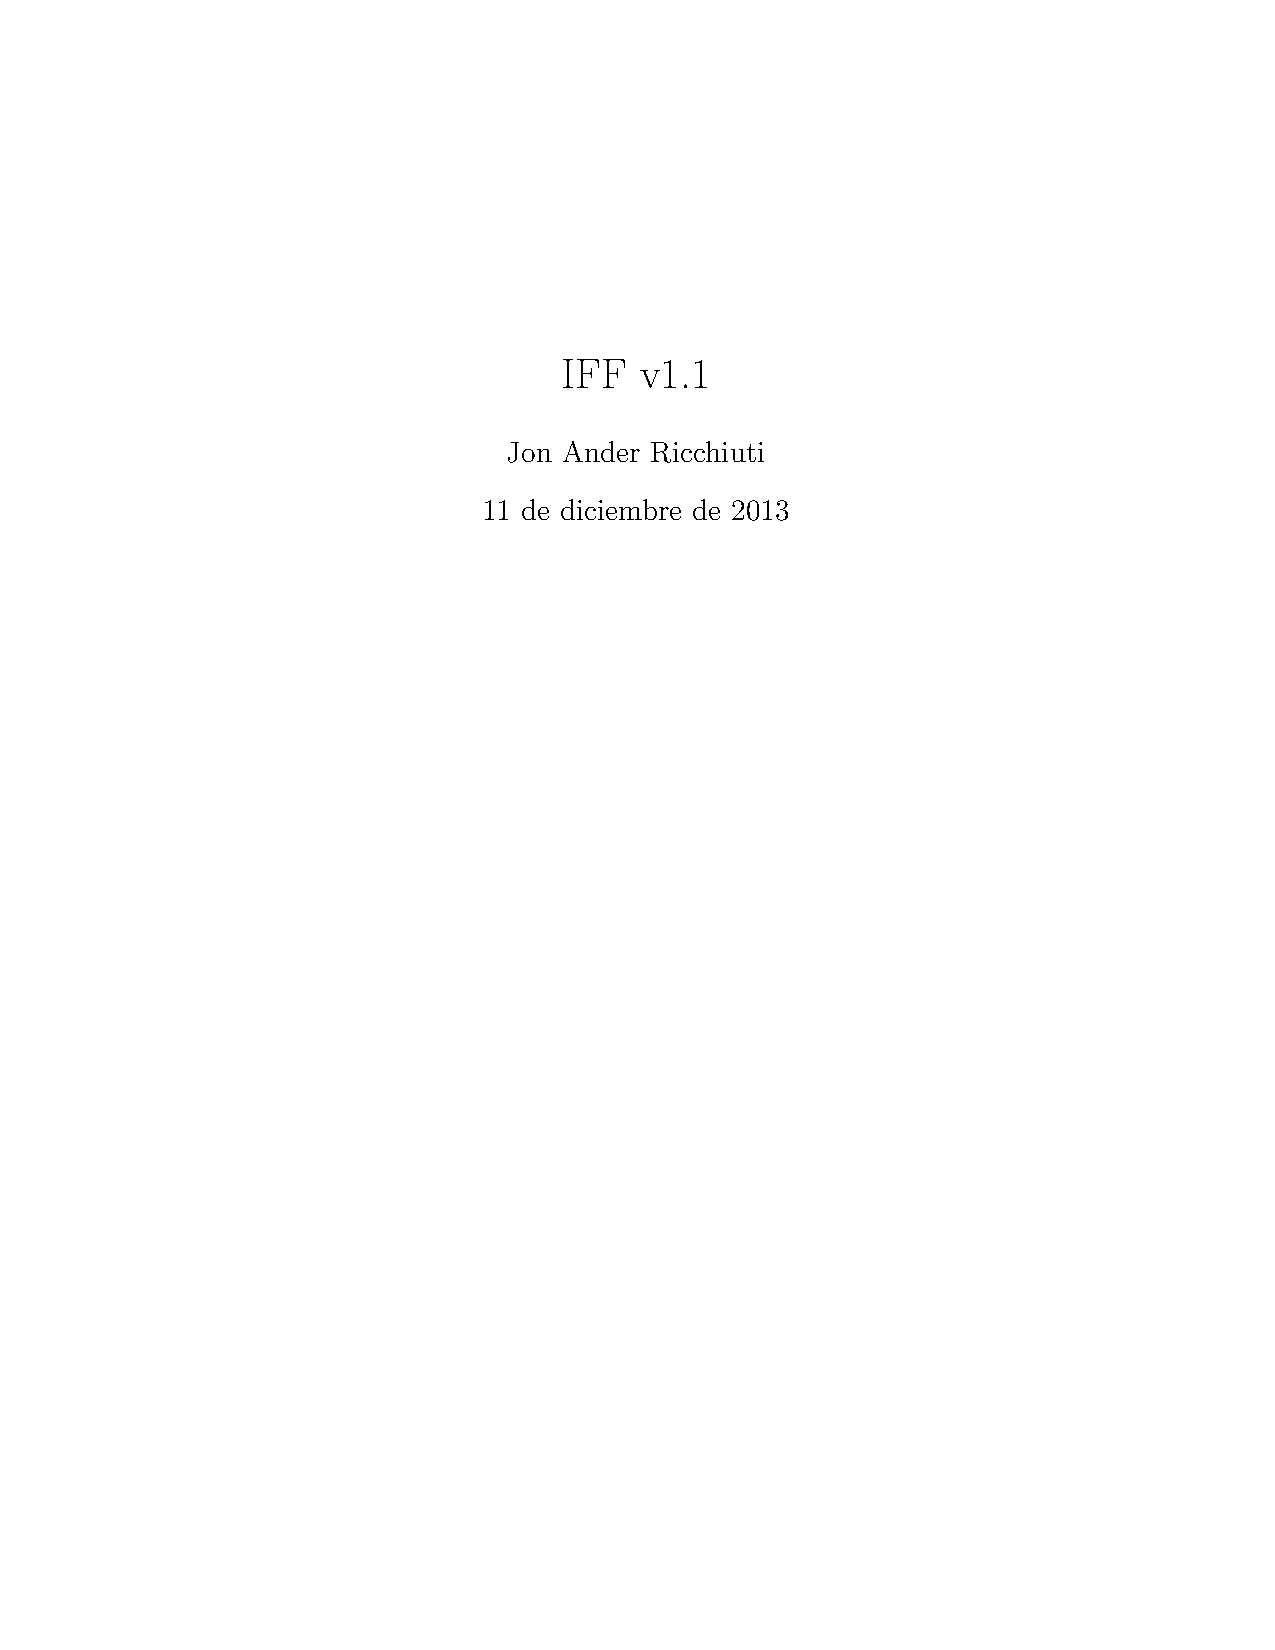
\includepdf[pages=-]{apendices/IFFv1.1/IFF.pdf}
%%\documentclass[12pt,letterpaper]{article}
%\usepackage[utf8]{inputenc}
%\usepackage{amsmath}
%\usepackage{amsfonts}
%\usepackage{amssymb}
%\usepackage[spanish]{babel}
%\usepackage{array}
%\usepackage{longtable}
%\author{Jon Ander Ricchiuti}
%\title{IFF v1.1}
%\begin{document}
%\pagenumbering{arabic}
%\maketitle
%\thispagestyle{empty}
%\newpage
\chapter{Intercambio de Información Financiera (IFF)}

\section*{Introducción}

El protocolo de intercambio de información financiera (IFF), describe la forma correcta de comunicación con un prototipo de sistema bancario creado en Synergy Global Business (SGB). El IFF busca estandarizar el intercambio de información financiera que realizará el prototipo bancario. De esta manera la comunicación es sencilla y a la vez robusta. Para la realización de este protocolo de comunicación se utilizó como base el IFX (Interactive Financial Exchange).
\\
\\ 
La forma de comunicación que el IFF	utiliza es de tipo petición-respuesta (request-response). En cada petición se debe especificar un método. Este método define la naturaleza de la petición.
%\pagenumbering{arabic}
%\newpage

\section{Tipo de datos}

Los tipos de datos que se utilizarán en este estándar son los siguientes:
\begin{itemize}
\item Cadena de caracteres.
\item Enumeración.
\item Tiempo y Hora.
\item Entero.
\item Decimal
\item Booleano.
\end{itemize}

\subsection{Cadena de caracteres}
Las cadenas de caracteres se representan con el nombre de ``Cadena de caracteres'' seguido de la longitud de la misma. Esta longitud es representada entre paréntesis de la siguiente forma.
\begin{itemize}
\item Cadena de caracteres (X-Y), indica que la longitud mínima de la cadena de caracteres es ``X'' y la máxima longitud es ``Y''.
\item Cadena de caracteres (X+), indica que la longitud mínima de la cadena de caracteres es ``X'' pero no tiene longitud máxima para la misma.
\end{itemize}
Si la longitud no es especificada entonces no existe restricción sobre el tamaño de la cadena de caracteres.

\subsection{Enumeración}
Son los valores que puede tomar un campo. Estos pertenecen a un conjunto de cadena de caracteres definidas específicamente para ese campo en particular. Los diferentes tipos de enumeración serán especificados en la siguiente sección.

\subsection{Tiempo y Hora}
Tanto la hora como la fecha son cadenas de caracteres que se representan con un fromato particular. Para la hora el formto es ``\%H:\%M:\%S''. Para la fecha el formato es ``\%Y-\%m-\%d \%H:\%M:\%S''. Donde \%Y representa el año, \%m el mes, \%d el dia, \%H la hora, \%M el minuto, \%S el segundo. Todos los componentes de la hora y fecha se representan con caracteres numéricos.

\subsection{Entero}
Es un número entero y puede representarse de dos formas diferentes. Como un entero de cuatro bytes o como un entero de ocho bytes. Para especificar que es un entero de ocho bytes, debe ser escrito de la siguiente forma: Entero(8).
\\
\\
Si no se especifica que un entero es de ocho bytes entonces se asume que es de cuatro  bytes.

\subsection{Decimal}
Es un número con hasta quince dígitos decimales.

\subsection{Booleano}
Un Booleano representa si una condición se cumple o no. En el caso del IFF un Booleano será representado por medio de un carácter. Es decir, el carácter 'T' será el que representa cuando un estado es cierto y 'F' será el valor de cuando el estado no se cumple.

\section{Tipos de Enumeración}
\subsection{Correspondiente a personVerifyType}
\begin{center}
\begin{tabular}{|>{\centering\arraybackslash}p{0.3\textwidth}|>{\centering\arraybackslash}p{0.3\textwidth}|>{\centering\arraybackslash}p{0.3\textwidth}|}
\hline 
\bfseries {Valor} & \bfseries {Descripción} & \bfseries {Por defecto} \\ 
\hline 
Passport & Pasaporte de crédito & N \\ 
\hline 
CI & Cedula de identidad & N \\
\hline 
\end{tabular} 
\end{center}

\subsection{Correspondiente a nameAddrType}
\begin{center}
\begin{tabular}{|>{\centering\arraybackslash}p{0.3\textwidth}|>{\centering\arraybackslash}p{0.3\textwidth}|>{\centering\arraybackslash}p{0.3\textwidth}|}
\hline 
\bfseries {Valor} & \bfseries {Descripción} & \bfseries {Por defecto} \\ 
\hline 
Customer & Es la dirección del cliente & N \\ 
\hline 
ShipTo & Dirección a la cual algo debería ser enviado por correo & N \\
\hline 
Delivery & Dirección a la cual serán enviadas las facturas en papel & N \\
\hline 
\end{tabular} 
\end{center}

\subsection{Correspondiente a addrType}
\begin{center}
\begin{tabular}{|>{\centering\arraybackslash}p{0.3\textwidth}|>{\centering\arraybackslash}p{0.3\textwidth}|>{\centering\arraybackslash}p{0.3\textwidth}|}
\hline 
\bfseries {Valor} & \bfseries {Descripción} & \bfseries {Por defecto} \\ 
\hline 
Seasonal & Habitación vacacional & N \\ 
\hline 
Primary & Habitación principal & N \\
\hline 
Secondary & Habitación secundaria & N \\
\hline
Business & Dirección de negocio & N \\
\hline 
\end{tabular} 
\end{center}

\subsection{Correspondiente a cardStatusCode}
\begin{center}
\begin{tabular}{|>{\centering\arraybackslash}p{0.3\textwidth}|>{\centering\arraybackslash}p{0.3\textwidth}|>{\centering\arraybackslash}p{0.3\textwidth}|}
\hline 
\bfseries {Valor} & \bfseries {Descripción} & \bfseries {Por defecto} \\ 
\hline 
Active & Activa & N \\ 
\hline 
Expired & Vencida & N \\
\hline 
Blocked & Bloqueada & N \\
\hline
\end{tabular} 
\end{center}

\subsection{Correspondiente a accountStatusCode}
\begin{center}
\begin{tabular}{|>{\centering\arraybackslash}p{0.3\textwidth}|>{\centering\arraybackslash}p{0.3\textwidth}|>{\centering\arraybackslash}p{0.3\textwidth}|}
\hline 
\bfseries {Valor} & \bfseries {Descripción} & \bfseries {Por defecto} \\ 
\hline 
Active & Activa & N \\ 
\hline 
Blocked & Bloqueada & N \\
\hline
\end{tabular} 
\end{center}

\subsection{Correspondiente a cardType}
\begin{center}
\begin{tabular}{|>{\centering\arraybackslash}p{0.3\textwidth}|>{\centering\arraybackslash}p{0.3\textwidth}|>{\centering\arraybackslash}p{0.3\textwidth}|}
\hline 
\bfseries {Valor} & \bfseries {Descripción} & \bfseries {Por defecto} \\ 
\hline 
Credit & Tarjeta de crédito & N \\ 
\hline 
Debit & Tarjeta de débito & N \\
\hline 
\end{tabular} 
\end{center}

\subsection{Correspondiente a brand}
\begin{center}
\begin{tabular}{|>{\centering\arraybackslash}p{0.3\textwidth}|>{\centering\arraybackslash}p{0.3\textwidth}|>{\centering\arraybackslash}p{0.3\textwidth}|}
\hline 
\bfseries {Valor} & \bfseries {Descripción} & \bfseries {Por defecto} \\ 
\hline 
Visa &  & N \\ 
\hline 
MasterCard &  & N \\
\hline 
\end{tabular} 
\end{center}

\subsection{Correspondiente a transType}
\begin{center}
\begin{tabular}{|>{\centering\arraybackslash}p{0.3\textwidth}|>{\centering\arraybackslash}p{0.3\textwidth}|>{\centering\arraybackslash}p{0.3\textwidth}|}
\hline 
\bfseries {Valor} & \bfseries {Descripción} & \bfseries {Por defecto} \\ 
\hline 
Withdrawal & Retiro & N \\ 
\hline 
Deposit & Deposito & N \\
\hline 
Transference & Transferencia & N \\
\hline
\end{tabular} 
\end{center}

\subsection{Correspondiente a acctType}
\begin{center}
\begin{tabular}{|>{\centering\arraybackslash}p{0.3\textwidth}|>{\centering\arraybackslash}p{0.3\textwidth}|>{\centering\arraybackslash}p{0.3\textwidth}|}
\hline 
\bfseries {Valor} & \bfseries {Descripción} & \bfseries {Por defecto} \\ 
\hline 
Saving & Ahorro & N \\ 
\hline 
Current & Corriente & N \\
\hline 
Loan & Préstamo & N \\
\hline
\end{tabular} 
\end{center}

\subsection{Correspondiente a contactInfo}
\begin{center}
\begin{tabular}{|>{\centering\arraybackslash}p{0.3\textwidth}|>{\centering\arraybackslash}p{0.3\textwidth}|>{\centering\arraybackslash}p{0.3\textwidth}|}
\hline 
\bfseries {Valor} & \bfseries {Descripción} & \bfseries {Por defecto} \\ 
\hline 
dayPhone & Teléfono de contacto durante el día & N \\
\hline 
evePhone & Teléfono de contacto durante la tarde & N \\
\hline 
dayFax & Fax de contacto durante el día & N \\
\hline
eveFax & Fax de contacto durante la tarde & N \\
\hline
emailAddr & Dirección de correo electrónica & N \\
\hline
\end{tabular} 
\end{center}
	
\section{Recursos}
El protocolo IFF esta basado en recursos. Los recursos son fuentes de información sobre las cuales se realizan las peticiones. Estos recursos son divididos en dos grandes grupos, los concretos y los abstractos.

\subsection{Recursos concretos}
Los recursos concretos son la representación directa del modelo de datos que expone el core bancario para ofrecer sus servicios. Este tipo de recursos es muy sencillo y son los que permiten realizar las operaciones más básicas. \\

A continuación se presentan los recursos concretos.

\subsubsection{Nombre de usuario ``login''}
Contiene la información que relaciona el nombre de usuario electrónico con su información  en la institución financiera.

\begin{center}
\begin{tabular}{|>{\centering\arraybackslash}p{0.2\textwidth}|>{\centering\arraybackslash}p{0.2\textwidth}|>{\centering\arraybackslash}p{0.2\textwidth}|>{\centering\arraybackslash}p{0.2\textwidth}|}
\hline 
\bfseries {Etiqueta} & \bfseries {Tipo} & \bfseries {Uso} & \bfseries {Descripción} \\ 
\hline 
username & Cadena de caracteres (6-20) & Requerido & ID de ingreso del cliente \\ 
\hline 
password & Cadena de caracteres (6+) & Opcional & Clave de ingreso \\ 
\hline 
custPermId & Cadena de caracteres (32+) & Requerido & ID permanente del cliente. Es asignado por la institución financiera para representar al cliente en el sistema \\ 
\hline 
\end{tabular}
\end{center}

\subsubsection{Cliente ``customer''}
Tiene la información que identifica inequívocamente a un cliente.

\begin{center}
\begin{longtable}{|>{\centering\arraybackslash}p{0.25\textwidth}|>{\centering\arraybackslash}p{0.2\textwidth}|>{\centering\arraybackslash}p{0.15\textwidth}|>{\centering\arraybackslash}p{0.2\textwidth}|}
\hline 
\bfseries {Etiqueta} & \bfseries {Tipo} & \bfseries {Uso} & \bfseries {Descripción} \\ 
\hline 
custPermId & Cadena de caracteres (32+) & Opcional & ID permanente del cliente. Es asignado por la institución financiera para representar al cliente en el sistema \\ 
\hline 
personId & Cadena de caracteres (32+) & Opcional & Relación al objeto ``person'' \\ 
\hline 
custLogin & Cadena de caracteres (6-20) & Opcional & ID permanente del cliente. Es asignado por la institución financiera para representar al cliente en el sistema \\ 
\hline 
personalIdent & Cadena de caracteres (8+) & Requerido & Identificación personal presentada por el cliente \\ 
\hline 
personVerifyType & Enumeración & Requerido & El tipo de documento con el cual se verifica la identidad del cliente \\ 
\hline
dtBCustomer & Fecha & Opcional & Momento en el cual la persona se vuelve cliente de la institución \\ 
\hline
dtLLogin & Fecha & Opcional & Último momento en el cual el cliente utiliza su cuenta \\ 
\hline
group & Cadena de caracteres (32+) & Opcional & Relaciona al cliente con el objeto ``grupo'' \\ 
\hline
\end{longtable}
\end{center}

\subsubsection{Información del banco ``bankInformation''}
Agrupa la información esencial de una agencia bancaria.

\begin{center}
\begin{longtable}{|>{\centering\arraybackslash}p{0.2\textwidth}|>{\centering\arraybackslash}p{0.2\textwidth}|>{\centering\arraybackslash}p{0.2\textwidth}|>{\centering\arraybackslash}p{0.2\textwidth}|}
\hline 
\bfseries {Etiqueta} & \bfseries {Tipo} & \bfseries {Uso} & \bfseries {Descripción} \\ 
\hline 
bankId & Cadena de caracteres (4+) & Opcional & ID que identifica a la agencia bancaria \\ 
\hline 
name & Cadena de caracteres & Opcional & Nombre de la agencia \\ 
\hline 
branchId & Cadena de caracteres & Opcional & ID que identifica a la sucursal \\ 
\hline 
branchName & Cadena de caracteres & Opcional & Nombre de la sucursal \\ 
\hline 
postAddr & Cadena de caracteres & Opcional & Dirección \\ 
\hline
city & Cadena de caracteres & Opcional & Ciudad \\ 
\hline
stateProv & Cadena de caracteres & Opcional & Estado o Provincia \\ 
\hline
postalCode &  Cadena de caracteres (4+) & Opcional & Código postal \\ 
\hline
country & Cadena de caracteres & Opcional & País \\ 
\hline
\end{longtable}
\end{center}

\subsubsection{Dirección ``address''}
Representa la dirección suministrada por el cliente.

\begin{center}
\begin{longtable}{|>{\centering\arraybackslash}p{0.2\textwidth}|>{\centering\arraybackslash}p{0.2\textwidth}|>{\centering\arraybackslash}p{0.2\textwidth}|>{\centering\arraybackslash}p{0.2\textwidth}|}
\hline 
\bfseries {Etiqueta} & \bfseries {Tipo} & \bfseries {Uso} & \bfseries {Descripción} \\ 
\hline 
addressId & Cadena de caracteres & Opcional & ID que identifica a la dirección \\ 
\hline 
custPermId & Cadena de caracteres (32+) & Requerido & ID permanente del cliente. Es asignado por la institución financiera para representar al cliente en el sistema \\
\hline 
nameAddrType & Enumeración & Requerido & Define el uso de la información suministrada \\ 
\hline 
addr & Cadena de caracteres & Opcional & Dirección \\ 
\hline
city & Cadena de caracteres & Opcional & Ciudad \\ 
\hline
stateProv & Cadena de caracteres & Opcional & Estado o Provincia \\ 
\hline
postalCode &  Cadena de caracteres (4+) & Opcional & Código postal \\ 
\hline
country & Cadena de caracteres & Opcional & País \\ 
\hline
addrType & Enumeración & Opcional & Define el tipo de dirección \\ 
\hline
startDt & Hora & Opcional & Hora de inicio \\ 
\hline
endDt & Hora & Opcional & Hora de fin \\ 
\hline
\end{longtable}
\end{center}

\subsubsection{Información de contacto ``contactInfo''}
Información suministrada por el cliente para poder ser contactado en caso de necesitarlo.

\begin{center}
\begin{longtable}{|>{\centering\arraybackslash}p{0.25\textwidth}|>{\centering\arraybackslash}p{0.2\textwidth}|>{\centering\arraybackslash}p{0.15\textwidth}|>{\centering\arraybackslash}p{0.2\textwidth}|}
\hline 
\bfseries {Etiqueta} & \bfseries {Tipo} & \bfseries {Uso} & \bfseries {Descripción} \\ 
\hline 
contactInfoId & Cadena de caracteres (32+) & Opcional & ID que identifica la información de contacto del cliente \\ 
\hline 
custPermId & Cadena de caracteres (32+) & Requerido & ID permanente del cliente. Es asignado por la institución financiera para representar al cliente en el sistema \\
\hline 
custContactPref & Enumeración & Requerido & Representa la manera en la cual el cliente será contactado \\ 
\hline 
prefTimeStart & Hora & Opcional & Hora a partir de la cual puede ser contactado \\ 
\hline
prefTimeEnd & Hora de caracteres & Opcional & Hora a partir de la cual ya no puede ser contactado \\ 
\hline
dayPhone & Cadena de caracteres & Opcional (ver descripción) & Teléfono de contacto durante el día. 
\\ & & & \\
& & & Este campo es requerido si ni ``evePhone'', ``dayFax'', ``eveFax'' o ``emailAddr'' es suministrado \\ 
\hline
evePhone & Cadena de caracteres & Opcional (ver descripción) & Teléfono de contacto durante la tarde. \\ & & & \\
& & & Este campo es requerido si ni ``dayPhone'', ``dayFax'', ``eveFax'' o ``emailAddr'' es suministrado \\ 
\hline
dayFax & Cadena de caracteres & Opcional (ver descripción) & Fax de contacto durante el día. \\ & & & \\
& & & Este campo es requerido si ni ``dayPhone'', ``evePhone'', ``eveFax'' o ``emailAddr'' es suministrado \\ 
\hline
eveFax & Cadena de caracteres & Opcional (ver descripción) & Fax de contacto durante la tarde. \\ & & & \\
& & & Este campo es requerido si ni ``dayPhone'', ``evePhone'', ``dayFax'' o ``emailAddr'' es suministrado \\ 
\hline
emailAddr & Cadena de caracteres & Opcional (ver descripción) & Correo electrónico de contacto. \\ & & & \\
& & & Este campo es requerido si ni ``dayPhone'', ``evePhone'', ``dayFax'' o ``eveFax'' es suministrado \\ 
\hline
\end{longtable}
\end{center}

\subsubsection{Información personal ``personalInfo''}
Contiene la información personal de un cliente.

\begin{center}
\begin{longtable}{|>{\centering\arraybackslash}p{0.2\textwidth}|>{\centering\arraybackslash}p{0.2\textwidth}|>{\centering\arraybackslash}p{0.2\textwidth}|>{\centering\arraybackslash}p{0.2\textwidth}|}
\hline 
\bfseries {Etiqueta} & \bfseries {Tipo} & \bfseries {Uso} & \bfseries {Descripción} \\ 
\hline 
personalInfoId & Cadena de caracteres (32+) & Opcional & ID que identifica a la información personal del cliente \\ 
\hline 
custPermId & Cadena de caracteres (32+) & Requerido & ID permanente del cliente. Es asignado por la institución financiera para representar al cliente en el sistema \\
\hline 
lastName & Cadena de caracteres & Requerido & Apellido del cliente \\ 
\hline 
firstName & Cadena de caracteres & Requerido & Dirección \\ 
\hline
middleName & Cadena de caracteres & Opcional & Ciudad \\ 
\hline
tittlePrefix & Cadena de caracteres & Opcional & Titulo por el cual llamar al cliente. Por ejemplo ``Dr.'' \\ 
\hline
nameSuffix & Cadena de caracteres & Opcional & Sufijo agregado al final del nombre del cliente. Por ejemplo ``Jr.'' \\ 
\hline
\end{longtable}
\end{center}

\subsubsection{Preferencia ``preference''}
Permite al cliente definir cierto comportamiento sobre su cuenta. El cliente puede establecer un monto predeterminado para concepto de retiro sobre una de sus cuentas. También, si se le ha hecho una transferencia al cliente y no se especificó cuenta destino, el dinero será transferido a la cuenta que el cliente haya definido por defecto.

\begin{center}
\begin{longtable}{|>{\centering\arraybackslash}p{0.3\textwidth}|>{\centering\arraybackslash}p{0.15\textwidth}|>{\centering\arraybackslash}p{0.15\textwidth}|>{\centering\arraybackslash}p{0.2\textwidth}|}
\hline 
\bfseries {Etiqueta} & \bfseries {Tipo} & \bfseries {Uso} & \bfseries {Descripción} \\ 
\hline 
preferenceId & Cadena de caracteres (32+) & Opcional & ID que identifica a la información de preferencia del cliente \\ 
\hline 
custPermId & Cadena de caracteres (32+) & Requerido & ID permanente del cliente. Es asignado por la institución financiera para representar al cliente en el sistema \\
\hline 
acctId & Cadena de caracteres (32+) & Opcional & ID de la cuenta a la cual se le aplicaran los consumos por concepto de retiros predefinidos \\ 
\hline 
defaultTranfAccount & Cadena de caracteres (32+) & Opcional & ID de la cuenta a la cual se le aplicaran las transferencias sin cuenta de destino especificada \\ 
\hline
withdrawalAmt & Cadena de caracteres (32+) & Opcional (ver descripción) & Monto de retiro por defecto. 
\\ & & & \\
& & & Este campo es requerido si ``acctId'' es especificado \\
\hline
\end{longtable}
\end{center}

\subsubsection{Transferencias a terceros ``registeredRecipient''}
Contiene los datos de alguna cuenta o tarjeta de otro banco junto con la identificación de sus acreedores.

\begin{center}
\begin{longtable}{|>{\centering\arraybackslash}p{0.25\textwidth}|>{\centering\arraybackslash}p{0.2\textwidth}|>{\centering\arraybackslash}p{0.15\textwidth}|>{\centering\arraybackslash}p{0.2\textwidth}|}
\hline 
\bfseries {Etiqueta} & \bfseries {Tipo} & \bfseries {Uso} & \bfseries {Descripción} \\ 
\hline 
recipientId & Cadena de caracteres (32+) & Opcional & ID que identifica la información acerca de un cliente en otra institución financiera \\ 
\hline 
custPermId & Cadena de caracteres (32+) & Requerido & ID permanente del cliente. Es asignado por la institución financiera para representar al cliente en el sistema \\
\hline 
personId & Cadena de caracteres (32+) & Opcional & ID que identifica al objeto ``person'' \\ 
\hline 
acctNum & Cadena de caracteres & Opcional (ver descripción) & representa el número de cuenta en alguna otra institución financiera. 
\\ & & & \\
& & & Este campo es requerido si ``cardSeqNum'' no es especificado \\ 
\hline
cardSeqNum & Cadena de caracteres & Opcional (ver descripción) & representa el número de tarjeta de alguna otra institución financiera. 
\\ & & & \\
& & & Este campo es requerido si ``acctNum'' no es especificado \\ 
\hline
name & Cadena de caracteres & Requerido & Nombre del beneficiario \\ 
\hline
desc & Cadena de caracteres & Requerido & Descripción \\ 
\hline
maxAmtLimit & Cadena de caracteres & Opcional & Máximo monto permitido para realizar la transferencia \\ 
\hline
personalIdent & Cadena de caracteres (8+) & Requerido & Identificación personal presentada por el cliente \\ 
\hline
personVerifyType & Enumeración & Requerido & El tipo de documento con el cual se verifica la identidad del cliente \\ 
\hline
\end{longtable}
\end{center}

\subsubsection{Persona ``person''}
Contiene los datos que identifican a los clientes como personas. También reúne los
datos de los clientes que tienen cuentas en otros bancos, estos datos provienen de
``registeredRecipient''.

\begin{center}
\begin{longtable}{|>{\centering\arraybackslash}p{0.3\textwidth}|>{\centering\arraybackslash}p{0.15\textwidth}|>{\centering\arraybackslash}p{0.15\textwidth}|>{\centering\arraybackslash}p{0.2\textwidth}|}
\hline 
\bfseries {Etiqueta} & \bfseries {Tipo} & \bfseries {Uso} & \bfseries {Descripción} \\ 
\hline 
personId & Cadena de caracteres (32+) & Opcional & ID que identifica a la información de una persona \\ 
\hline 
name & Cadena de caracteres & Requerido & Nombre \\
\hline 
\end{longtable}
\end{center}

\subsubsection{Conocido ``known''}
Contiene la información de las personas conocidas. De esta forma se puede pueden
realizar transferencias a personas en lugar de a cuentas.

\begin{center}
\begin{longtable}{|>{\centering\arraybackslash}p{0.3\textwidth}|>{\centering\arraybackslash}p{0.15\textwidth}|>{\centering\arraybackslash}p{0.15\textwidth}|>{\centering\arraybackslash}p{0.2\textwidth}|}
\hline 
\bfseries {Etiqueta} & \bfseries {Tipo} & \bfseries {Uso} & \bfseries {Descripción} \\ 
\hline 
knownId & Cadena de caracteres (32+) & Opcional & ID que identifica a la información acerca de un conocido	 \\ 
\hline 
personId & Cadena de caracteres (32+) & Requerido & ID que identifica la información acerca de una persona.
\\ & & & \\
& & & En este caso representa a un conocido \\
\hline 
custPermId & Cadena de caracteres (32) & Requerido & ID permanente del cliente. Es asignado por la institución financiera para representar al cliente en el sistema.
\\ & & & \\
& & & En este caso representa al conocedor \\
\hline 
relationship & Cadena de caracteres & Requerido & Describe el tipo de relación entre el conocedor y el conocido. \\ 
\hline 
status & Booleano & Opcional & Representa si se ha validado que estas dos personas se conocen \\ 
\hline 
\end{longtable}
\end{center}

\subsubsection{Miembro de un grupo ``groupMember''}
Un cliente tiene la capacidad de crear grupo de personas conocidas. De esta forma puede establecer en que cuenta serán ubicados los fondos recibidos por parte de algún miembro del grupo. Un miembro del grupo es aquel cliente que pertenezca a un grupo.

\begin{center}
\begin{longtable}{|>{\centering\arraybackslash}p{0.25\textwidth}|>{\centering\arraybackslash}p{0.2\textwidth}|>{\centering\arraybackslash}p{0.15\textwidth}|>{\centering\arraybackslash}p{0.2\textwidth}|}
\hline 
\bfseries {Etiqueta} & \bfseries {Tipo} & \bfseries {Uso} & \bfseries {Descripción} \\ 
\hline 
groupMemberId & Cadena de caracteres (32+) & Opcional & ID que identifica al objeto ``groupMember'' \\ 
\hline 
custPermId & Cadena de caracteres (32+) & Requerido & ID permanente del cliente. Es asignado por la institución financiera para representar al cliente en el sistema \\
\hline 
member & Cadena de caracteres (32+) & Requerido & Representa al cliente miembro del grupo \\
\hline 
groupId & Cadena de caracteres (32+) & Requerido & Identifica al grupo al cual pertenece un miembro de grupo\\
\hline 
\end{longtable}
\end{center}

\subsubsection{Grupo ``group''}
Es una unidad en la cual un cliente puede agrupar a otros clientes del banco y
predefinir una cuenta en la cual los miembros al grupo transferirán.

\begin{center}
\begin{longtable}{|>{\centering\arraybackslash}p{0.2\textwidth}|>{\centering\arraybackslash}p{0.2\textwidth}|>{\centering\arraybackslash}p{0.2\textwidth}|>{\centering\arraybackslash}p{0.2\textwidth}|}
\hline 
\bfseries {Etiqueta} & \bfseries {Tipo} & \bfseries {Uso} & \bfseries {Descripción} \\ 
\hline 
groupId & Cadena de caracteres (32+) & Opcional & ID que identifica al objeto ``group'' \\ 
\hline
acctId & Cadena de caracteres (32+) & Opcional & ID de la cuenta a la cual se le aplicaran los consumos por concepto de retiros predefinidos \\ 
\hline 
name & Cadena de caracteres & Requerido & Nombre del grupo \\
\hline 
descripción & Cadena de caracteres & Opcional & Descripción del grupo \\
\hline 
\end{longtable}
\end{center}

\subsubsection{Estado de la cuenta ``accountStatus''}
Tiene la información del estado en el cual se encuentra la cuenta.

\begin{center}
\begin{longtable}{|>{\centering\arraybackslash}p{0.25\textwidth}|>{\centering\arraybackslash}p{0.2\textwidth}|>{\centering\arraybackslash}p{0.15\textwidth}|>{\centering\arraybackslash}p{0.2\textwidth}|}
\hline 
\bfseries {Etiqueta} & \bfseries {Tipo} & \bfseries {Uso} & \bfseries {Descripción} \\ 
\hline 
accountStatusId & Cadena de caracteres (32+) & Opcional & ID que identifica al objeto ``accountStatus'' \\ 
\hline
acctId & Cadena de caracteres (32+) & Opcional & ID de la cuenta a la cual se le aplicaran los consumos por concepto de retiros predefinidos \\ 
\hline 
accountStatusCode & Enumeración & Requerido & Representa el estado de la cuenta \\
\hline 
effDt & Fecha & Opcional & Fecha en la cual se hizo efectivo dicho estado \\
\hline 
statusModBy & Cadena de caracteres & Opcional & Tiene la información acerca de quien modificó el estado \\
\hline 
statusDesc & Cadena de caracteres & Opcional & Descripción sobre el estado \\
\hline 
\end{longtable}
\end{center}

\subsubsection{Estado de la tarjeta ``cardStatus''}
Contiene la información del estado en el cual se encuentra la tarjeta.

\begin{center}
\begin{longtable}{|>{\centering\arraybackslash}p{0.25\textwidth}|>{\centering\arraybackslash}p{0.2\textwidth}|>{\centering\arraybackslash}p{0.15\textwidth}|>{\centering\arraybackslash}p{0.2\textwidth}|}
\hline 
\bfseries {Etiqueta} & \bfseries {Tipo} & \bfseries {Uso} & \bfseries {Descripción} \\ 
\hline 
card	StatusId & Cadena de caracteres (32+) & Opcional & ID que identifica al objeto ``cardStatus'' \\ 
\hline
cardEmBossNum & Cadena de caracteres (32+) & Requerido & Número de la tarjeta a la cual pertenece el estado \\ 
\hline 
cardStatusCode & Enumeración & Requerido & Representa el estado de la tarjeta \\
\hline 
effDt & Fecha & Opcional & Fecha en la cual se hizo efectivo dicho estado \\
\hline 
statusModBy & Cadena de caracteres & Opcional & Tiene la información acerca de quien modificó el estado \\
\hline 
statusDesc & Cadena de caracteres & Opcional & Descripción sobre el estado \\
\hline 
\end{longtable}
\end{center}

\subsubsection{Tarjeta ``card''}
Contiene la información de la tarjeta.

\begin{center}
\begin{longtable}{|>{\centering\arraybackslash}p{0.25\textwidth}|>{\centering\arraybackslash}p{0.2\textwidth}|>{\centering\arraybackslash}p{0.15\textwidth}|>{\centering\arraybackslash}p{0.2\textwidth}|}
\hline 
\bfseries {Etiqueta} & \bfseries {Tipo} & \bfseries {Uso} & \bfseries {Descripción} \\ 
\hline 
cardEmBossNum & Cadena de caracteres (32+) & Requerido & Número de la tarjeta \\ 
\hline
acctId & Cadena de caracteres (32+) & Requerido & ID de la cuenta a la cual se le aplicaran los consumos por concepto de retiros predefinidos \\ 
\hline
cardType & Enumeración & Opcional & Tipo de tarjeta \\
\hline 
brand & Enumeración & Opcional & Consorcio al que pertenece la tarjeta \\
\hline 
issuerName & Cadena de caracteres & Opcional & Nombre del tarjetahabiente \\
\hline 
issDt & Fecha & Opcional & Fecha en la cual se emite la tarjeta \\
\hline 
expDt & Fecha & Opcional & Fecha en la cual expira la tarjeta \\
\hline 
\end{longtable}
\end{center}

\subsubsection{Balance ``balance''}
Contiene la información del dinero existente en una cuenta y las transacciones que
la han afectado.

\begin{center}
\begin{longtable}{|>{\centering\arraybackslash}p{0.2\textwidth}|>{\centering\arraybackslash}p{0.2\textwidth}|>{\centering\arraybackslash}p{0.2\textwidth}|>{\centering\arraybackslash}p{0.2\textwidth}|}
\hline 
\bfseries {Etiqueta} & \bfseries {Tipo} & \bfseries {Uso} & \bfseries {Descripción} \\ 
\hline 
acctId & Cadena de caracteres (32+) & Requerido & ID de la cuenta a la cual pertenece el balance \\ 
\hline
transId & Entero (8) & Opcional & ID de la transacción que afectó el balance \\
\hline 
curAmt & Decimal & Requerido & Cantidad de dinero en la cuenta para la fecha \\
\hline 
effDt & Fecha & requerido & Fecha en la cual se afectó el balance \\
\hline 
descr & Cadena de caracteres & Opcional & Descripción \\
\hline 
\end{longtable}
\end{center}

\subsubsection{Transacción ``transaction''}
Cualquier movimiento que afecte algún balance.

\begin{center}
\begin{longtable}{|>{\centering\arraybackslash}p{0.2\textwidth}|>{\centering\arraybackslash}p{0.2\textwidth}|>{\centering\arraybackslash}p{0.2\textwidth}|>{\centering\arraybackslash}p{0.2\textwidth}|}
\hline 
\bfseries {Etiqueta} & \bfseries {Tipo} & \bfseries {Uso} & \bfseries {Descripción} \\ 
\hline
transId & Entero (8) & Opcional & ID de la transacción \\
\hline 
acctId & Cadena de caracteres (32+) & Requerido & ID de la cuenta que realizó la transacción \\ 
\hline 
acctOutFlow & Cadena de caracteres (32+) & Opcional (ver descripción) & ID de la cuenta a la cual se le debitará el dinero.
\\ & & & \\
& & & Este campo es requerido en caso de que la transacción debite de alguna forma dinero de la cuenta \\
\hline 
acctInFlow & Cadena de caracteres (32+) & Opcional (ver descripción) & ID de la cuenta que recibirá el dinero.
\\ & & & \\
& & & Este campo es requerido en caso de que la transacción abone de alguna forma dinero a la cuenta \\
\hline
thirdParty & Cadena de caracteres & Opcional (ver descripción) & ID de la cuenta o tarjeta de un beneficiario en otro banco.
\\ & & & \\
& & & Este campo es requerido en caso de existir un tercero involucrado \\
\hline
amt & Decimal & Requerido & Cantidad de dinero que moverá la transacción \\
\hline 
dueDt & Fecha & Requerido & Fecha en la cual se desea la transacción sea efectuada \\
\hline 
curDt & Fecha & Requerido & Fecha en la cual se realizó la transacción \\
\hline 
transType & Enumeración & Opcional & Tipo de transacción realizada \\
\hline 
\end{longtable}
\end{center}

\subsubsection{Transacción ``transaction''}
Cualquier movimiento que afecte algún balance.

\begin{center}
\begin{longtable}{|>{\centering\arraybackslash}p{0.2\textwidth}|>{\centering\arraybackslash}p{0.2\textwidth}|>{\centering\arraybackslash}p{0.2\textwidth}|>{\centering\arraybackslash}p{0.2\textwidth}|}
\hline 
\bfseries {Etiqueta} & \bfseries {Tipo} & \bfseries {Uso} & \bfseries {Descripción} \\ 
\hline
acctId & Cadena de caracteres (32+) & Requerido & ID de la cuenta que realizó la transacción \\ 
\hline 
bankId & Cadena de caracteres & Requerido & ID que identifica a la agencia bancaria \\
\hline 
custPermId & Cadena de caracteres (32+) & Requerido & ID permanente del cliente. Es asignado por la institución financiera para representar al cliente en el sistema 
\\ & & & \\
& & & Este campo es requerido si la cuenta no es compartida \\
\hline
acctType & Enumeración & Requerido & Define de qué tipo es la cuenta \\
\hline
freeForAll & Booleano & Opcional (ver descripción) & En caso de que la cuenta sea compartida, define si cualquiera puede efectuar operaciones o se necesita la aprobación de todos los participantes.
\\ & & & \\
& & & Es requerido si el campo ``custPermId'' no está definido \\
\hline 
members & Entero & Opcional (ver descripción) & Define cuantos clientes comparten la cuenta
\\ & & & \\
& & & El campo es requerido si ``freeForAll'' está definido \\
\hline 
\end{longtable}
\end{center}

\subsection{Recursos abstractos}
A diferencia de los recursos concretos, los recursos abstractos no representan objetos en la base de datos. Estos recursos ofrecen una información más general y son producto de una recopilación de información sobre varios objetos en la base de datos. También se pueden utilizar estos recursos para ofrecer una forma más sencilla de actualizar alguna información en el sistema. Por ejemplo, si se desea registrar un nuevo cliente, se tendrían que mandar varias peticiones para crear los recursos necesarios para que el cliente sea registrado. Para evitar mandar varias peticiones se podría ofrecer un recurso que recopile toda la información necesaria y este se encargue de crear los recursos concretos necesarios para que el nuevo cliente pueda ser registrado.
%\end{document}
%\chapter{Ejemplos del lenguaje}\label{ejemplos_lenguaje}

Estos ejemplos quieren ilustrar el uso de la herramienta en las distintas áreas de la 
computación.

\section{Caso 1: Base de datos}
\label{ejemplo:bd}
En este caso se quiere crear objetos que representan a 5 personas para una base 
de datos cuya única restricción es que sus cédulas aparezcan de mayor a menor. 
Los datos que tiene cada persona pueden ser:

\begin{itemize}
\item{La cédula que va desde 1000 a 1100.}
\item{El nombre que puede ser alguno de estos: Juan, Pedro, Marco, Jose, Isaac, Tony, Alexis, Erick, Hancel, Alfredo o Carlos.}
\item{Y finalmente el nombre de la bebida que le gusta, que puede ser alguna de estas: Agua, Té, Pepsi, CocaCola o Nestea.}
\end{itemize}

\begin{lstlisting}[mathescape]
salida personas {
 descripcion {
  persona p1;
  persona p2;
  persona p3;
  persona p4;
  persona p5;
 }
 restriccion {
  p1.cedula > p2.cedula;
  p2.cedula > p3.cedula;
  p3.cedula > p4.cedula;
  p4.cedula > p5.cedula;
 }
}

aux persona {
 descripcion {
  int (1000, 1100) cedula;
  Str nombre =$\sim$ ["Juan" | "Pedro" | "Jose" | "Isaac" | "Tony" | 
            "Alexis" | "Erick" | "Hancel" | "Alfredo" | "Carlos" | "Marco"];
  Str bebida =$\sim$ ["Agua" | "Te" | "Pepsi" | "CocaCola" | "Nestea"];
 }
}
\end{lstlisting}

\section{Caso 2: Computación gráfica}
\label{ejemplo:cg}
Para este ejemplo se quiere crear escenarios con casas aleatorias y los datos de estas son:

\begin{itemize}
\item{Número de pisos que pueden ser entre 1 y 3.}
\item{Altura de los pisos que debe ser un flotante entre 2 y 3.}
\item{Ancho y profundidad de la casa que esta entre 10 y 20.}
\item{Un booleano que indique que si la casa tiene chimenea o no.}
\end{itemize}

\begin{lstlisting}[mathescape]
salida casa {
 descripcion { 
  int (1,3) pisos; 
  float (2,3) alturaPiso; 
  float (10,20) ancho; 
  float (10,20) profundidad; 
  bool chimenea; 
 } 
}
\end{lstlisting}

\section{Caso 3: HTML}
\label{ejemplo:html}
Para este caso lo que se quiere es probar distintas alturas de \emph{header}, \emph{content}
y \emph{footer} dentro de una página web, la única retricción que que tienen en 
común es que tengan el mismo ancho y los valores que admite estan entre 750 y 800.
Las restricciones en particular cada una de estas partes son:

\begin{itemize}
\item{\emph{Header} tiene un alto que puede ser alguno de estos valores 100, 150, 200, 250 y 300.}
\item{\emph{Content} tiene un alto que puede ser entre 500 y 800.}
\item{\emph{Footer} tiene un alto que puede ser entre 50 y 100.}
\end{itemize}

\begin{lstlisting}[mathescape]
salida html { 
 descripcion { 
  header  parte1;
  content parte2; 
  footer  parte3; 
 } 
 restriccion { 
  parte1.width == parte2.width; 
  parte1.width == parte3.width; 
 } 
} 
aux header { 
 descripcion { 
  int height $=\sim$ [100 $\mid$ 150 $\mid$ 200 $\mid$ 250 $\mid$ 300]; 
  int (750,800) width; 
 } 
} 
aux content { 
 descripcion { 
  int (500,800) height; 
  int (750,800) width; 
 } 
}
aux footer {
 descripcion { 
  int (50,100) height; 
  int (750,800) width; 
 } 
}
\end{lstlisting}

%\chapter{Especificación formal de la sintaxis}\label{gramaticas_lenguaje}

Para reconocer el lenguaje propuesto en la sección \ref{chapter:def_lenguaje},
se crearon las gramáticas que están en la sección \ref{gramaticas_lenguaje_detalle}
y los tokens correspondientes a estas últimas se encuentran en la sección 
\ref{tokens_lenguaje_detalle}.

\section{Gramáticas} \label{gramaticas_lenguaje_detalle}

\begin{lstlisting}[mathescape]
principal:
  definicion TKEXIT TKID TKLBRACE descripcion restriccion TKRBRACE definicion

definicion:
  definicion TKAUXILIAR TKID TKLBRACE descripcion restriccion TKRBRACE
  |definicion TKFUNCTIONS TKLBRACE funciones TKRBRACE
  |

descripcion:
  TKDESCRIPTION TKLBRACE declaracion_variable TKRBRACE 

restriccion:
  TKRESTRICTION lista_bloque_restricciones porcentaje 
  |

lista_bloque_restricciones:
  bloque_restricciones
  |lista_bloque_restricciones operador_logico_simple bloque_restricciones 

bloque_restricciones:
  operador_unario bloque_restricciones 
  |TKLBRACE lista_sub_bloque_restricciones TKRBRACE 
  |TKLBRACKET lista_sub_bloque_restricciones TKRBRACKET 

lista_sub_bloque_restricciones:
  lista_sub_bloque_restricciones_operados porcentaje TKSEMICOLON 
  |lista_sub_bloque_restricciones lista_sub_bloque_restricciones_operados porcentaje TKSEMICOLON 

lista_sub_bloque_restricciones_operados:
  sub_bloque_restricciones 
  |lista_sub_bloque_restricciones_operados operador_logico_simple sub_bloque_restricciones 

sub_bloque_restricciones:
  bloque_restricciones 
  |expresion
  |distribucion 
  |cuantificador 
  |operador_unario cuantificador 

declaracion_variable:
  anulable tipo_variable rango_random TKID asignacion TKSEMICOLON 
  |declaracion_variable anulable tipo_variable rango_random TKID asignacion TKSEMICOLON 

rango_random:
  TKLPARENTHESES negativo TKINTVALUE TKCOMMA negativo TKINTVALUE TKRPARENTHESES
  |TKLPARENTHESES negativo TKFLOATVALUE TKCOMMA negativo TKINTVALUE TKRPARENTHESES
  |TKLPARENTHESES negativo TKINTVALUE TKCOMMA negativo TKFLOATVALUE TKRPARENTHESES
  |TKLPARENTHESES negativo TKFLOATVALUE TKCOMMA negativo TKFLOATVALUE TKRPARENTHESES
  |

negativo:
  TKHYPHEN
  |

anulable:
  TKIGNORE  
  |

tipo_variable:
  TKBOOL      
  |TKINT      
  |TKCHAR     
  |TKFLOAT    
  |TKSTRING   
  |TKDOUBLE   
  |TKVECTOR2  
  |TKVECTOR3  
  |TKVECTOR4
  |TKLIST TKLESSTHAN tipo_variable TKMORETHAN
  |TKID
  
asignacion:
  TKEQUAL expresion
  |TKEQUAL TKTILDE TKLBRACKET opciones TKRBRACKET 
  |TKTILDE lista_bloque_restricciones porcentaje  
  |
  
expresion:
  tipos_basicos 
  |variable_mixta 
  |operador_unario expresion
  |expresion operador_binario expresion
  |TKLPARENTHESES expresion TKRPARENTHESES 
  |llamada_funcion 
  |TKLBRACKET elemento_lista TKRBRACKET 
  |TKLBRACKET TKRBRACKET 
  |TKLPARENTHESES expresion TKCOMMA expresion TKRPARENTHESES
  |TKLPARENTHESES expresion TKCOMMA expresion TKCOMMA expresion TKRPARENTHESES
  |TKLPARENTHESES expresion TKCOMMA expresion TKCOMMA expresion TKCOMMA expresion TKRPARENTHESES 
  |TKNULL 
  |expresion operador_logico expresion
  |expresion operador_binario_matematico_logico expresion

variable_mixta:
  variable_acceso 
  |variable_acceso TKLBRACKET expresion TKRBRACKET accesos 
  |TKNUMBERSIGN 
  |TKNUMBERSIGN TKDOT variable_acceso 
  |TKNUMBERSIGN TKLBRACKET expresion TKRBRACKET accesos 
  |TKNUMBERSIGN TKDOT variable_acceso TKLBRACKET expresion TKRBRACKET accesos 

variable_acceso:
  TKID                        
  |variable_acceso TKDOT TKID 

accesos:
  accesos TKDOT variable_acceso TKLBRACKET expresion TKRBRACKET 
  | 

operador_unario:
  TKHYPHEN  
  |TKNEGATE 

operador_binario:
  TKHYPHEN    
  |TKPLUS     
  |TKASTERISK 
  |TKSLASH    
  |TKPERCENT  
  |TKCARET    

opciones:
  tipos_basicos porcentaje 
  |opciones TKBAR tipos_basicos porcentaje 

tipos_basicos:
  TKSTRINGVALUE 
  |TKTRUE       
  |TKFALSE      
  |TKINTVALUE   
  |TKFLOATVALUE 
  |TKDOUBLEVALUE 
  |TKCHARVALUE  

porcentaje:
  TKINTVALUE TKPERCENT 
  |TKFLOATVALUE TKPERCENT 
  | 

llamada_funcion:
  TKID TKLPARENTHESES parametro_funcion TKRPARENTHESES 

parametro_funcion:
  expresion  
  |parametro_funcion TKCOMMA expresion 

operador_logico:
  operador_logico_simple  
  |TKAND                  
  |TKOR                   

operador_logico_simple:
  TKEQUIVALENT            
  |TKIMPLICATION          
  |TKCONSECUENCE          
  |TKDISTINCT             

operador_binario_matematico_logico:
  TKLESSTHAN              
  |TKMORETHAN             
  |TKLESSEQUALTHAN        
  |TKMOREEQUALTHAN        
  |TKEQUAL                

elemento_lista:
  expresion 
  |elemento_lista TKCOMMA expresion 

distribucion:
  variable_mixta TKTILDE llamada_funcion 

cuantificador:
  TKFOR operador_cuantificador TKLPARENTHESES lista_variables TKRPARENTHESES TKTILDE lista_bloque_restricciones

operador_cuantificador:
  TKANY                   
  |TKALL                  
  |TKATMOST TKINTVALUE    
  |TKATLEAST TKINTVALUE   
  |TKEXACTLY TKINTVALUE   

lista_variables:
  TKID TKFROM variable_mixta 
  |lista_variables TKCOMMA TKID TKFROM variable_mixta 

funciones:
  funcion_firma 
  |funciones funcion_firma

funcion_firma:
  tipo_variable TKID TKLPARENTHESES firma_parametros TKRPARENTHESES TKEQUAL variables_aleatorias expresion_funciones

firma_parametros:
  par_tipo_nombre 
  |

par_tipo_nombre:
  tipo_variable TKID 
  |par_tipo_nombre TKCOMMA tipo_variable TKID 

variables_aleatorias:
  TKVARIABLES TKLBRACE declaracion_variable TKRBRACE TKIN 
  | 

expresion_funciones:
  expresion 
  |TKIF TKLPARENTHESES expresion TKRPARENTHESES TKTHEN expresion_funciones else_if TKELSE expresion_funciones 

else_if:
  else_if TKELSEIF TKLPARENTHESES expresion TKRPARENTHESES TKTHEN expresion_funciones 
  | 
\end{lstlisting}

\section{Tokens}\label{tokens_lenguaje_detalle}

Los tokens que se definieron para el lenguaje se clasificaron en 3 grupos.

\begin{table}[h]
\centering
\begin{tabular}{|c|c|c|c|}
\hline
Símbolo & Token & Símbolo & Token \\
\hline
\{     & TKLBRACE &  !     & TKNEGATE  \\
\hline
\}     & TKRBRACE & ;     & TKSEMICOLON \\
\hline
[     & TKLBRACKET & *     & TKASTERISK \\
\hline
]     & TKRBRACKET & $<$     & TKLESSTHAN \\
\hline
(     & TKLPARENTHESES & $>$     & TKMORETHAN \\
\hline
)     & TKRPARENTHESES & =     & TKEQUAL \\
\hline
$\sim$     & TKTILDE & !=   & TKDISTINCT \\
\hline
\end{tabular}
\caption{Tokens de símbolos 1}\label{tab:tok_simb_1}
\end{table}

\begin{table}[h]
\centering
\begin{tabular}{|c|c|c|c|}
\hline
Símbolo & Token & Símbolo & Token \\
\hline
\#     & TKNUMBERSIGN & ,     & TKCOMMA\\
\hline
-     & TKHYPHEN & +     & TKPLUS\\
\hline
/     & TKSLASH  & \%     & TKPERCENT\\
\hline
$\wedge$  & TKCARET & $\mid$ & TKBAR\\
\hline
.     & TKDOT & 	\textdollar  & TKIGNORE \\
\hline
$==$   & TKEQUALEQUAL & === & TKEQUIVALENT \\
\hline
$==>$ & TKIMPLICATION & $<==$ & TKCONSECUENCE\\
\hline
\&\&   & TKAND & $\mid\mid$   & TKOR \\
\hline
$<=$   & TKLESSEQUALTHAN & $>=$   & TKMOREEQUALTHAN \\
\hline
$<-$   & TKFROM & ~ & ~ \\
\hline
\end{tabular}
\caption{Tokens de símbolos 2}\label{tab:tok_simb_2}
\end{table}

\begin{table}[h]
\centering
\begin{tabular}{|c|c|}
\hline
Expresión regular & Token \\
\hline
$0|[1-9][0-9]*$ & TKINTVALUE \\
\hline
$0.[0-9]+|[1-9][0-9]*.[0-9]+$ & TKFLOATVALUE\\
\hline
$0.[0-9]+|[1-9][0-9]*.[0-9]+$ & TKDOUBLEVALUE\\
\hline
[a-zñá-úä-üA-ZÑÁ-ÚÄ-Ü\_]+ & TKID \\
\hline
``.*'' & TKSTRINGVALUE \\
\hline
'.'  & TKCHARVALUE \\
\hline
\end{tabular}
\caption{Tokens de valores}\label{tab:tok_valores}
\end{table}

\begin{table}[h]
\centering
\begin{tabular}{|c|c|c|}
\hline
Expresión regular inglés & Expresión regular español & Token \\
\hline
exit & salida & TKEXIT \\
\hline
functions & funciones & TKFUNCTIONS \\
\hline
aux & auxiliar & TKAUXILIAR \\
\hline
description & descripcion & TKDESCRIPTION \\
\hline
restriction & restriccion & TKRESTRICTION \\
\hline
entero & int    & TKINT \\
\hline
bool  & bool & TKBOOL \\
\hline
char   & caracter & TKCHAR \\
\hline
float  & flotante &  TKFLOAT \\
\hline
Double & Doble  & TKDOUBLE \\
\hline
Str    & Caracteres & TKSTRING \\
\hline
vector2 & vector2 &TKVECTOR2 \\
\hline
vector3 & vector3 &TKVECTOR3 \\
\hline
vector4 & vector4 &TKVECTOR4 \\
\hline
list   & lista  & TKLIST \\
\hline
for    & para   & TKFOR \\
\hline
any    & algun  & TKANY \\
\hline
all    & todos  & TKALL \\
\hline
at\ most & a\ lo\ sumo & TKATMOST \\
\hline
at\ least & al\ menos & TKATLEAST \\
\hline
exactly & exactamente & TKEXACTLY \\
\hline
variables & variables & TKVARIABLES \\
\hline
in     & en     & TKIN \\
\hline
if     & si     & TKIF \\
\hline
then   & entonces & TKTHEN \\
\hline
elseif & si\_en\_vez &  TKELSEIF \\
\hline
else   & si\_no & TKELSE \\
\hline
null   & nulo   & TKNULL \\
\hline
true   & verdadero & TKTRUE \\
\hline
false  & falso  & TKFALSE \\
\hline
\end{tabular}
\caption{Tokens de palabras reservadas}\label{tab:tok_palabras}
\end{table}


%\printglossary

\end{document}
